\section{Baseline Results}

This section reports the baseline performance of the trained classifier evaluated on a held-out test set
containing data from patients unseen during training and validation. All results presented here therefore
reflect patient-level generalisation performance rather than image-level memorisation.

Given the clinical context of breast cancer screening, a conservative operating point was selected.
Rather than using the default decision threshold of 0.5, the classification threshold was adjusted to
achieve approximately 90\% specificity. This reflects a screening-oriented deployment scenario in which
limiting false positive cases is important to reduce unnecessary follow-up investigations and patient
anxiety, while still retaining reasonable sensitivity. The resulting threshold was approximately
$\tau \approx 0.620$.

Table~\ref{tab:baseline_metrics} summarises the primary performance metrics achieved at this
specificity-constrained operating point. In addition to aggregate metrics such as ROC--AUC and average
precision, clinically interpretable measures including sensitivity, specificity, and the confusion matrix
counts are reported.

\begin{table}[H]
\centering
\begin{tabular}{lr}
\toprule
Metric & Value \\
\midrule
Decision threshold (spec $\approx$ 0.90) & 0.6205 \\
ROC--AUC & 0.7454 \\
Average Precision (AP) & 0.5996 \\
Precision & 0.6413 \\
Recall / Sensitivity & 0.3189 \\
Specificity & 0.9065 \\
F1-score & 0.4260 \\
\midrule
TP / FP / TN / FN & 59 / 33 / 320 / 126 \\
\bottomrule
\end{tabular}
\caption{Baseline test performance at the specificity-constrained operating point.}
\label{tab:baseline_metrics}
\end{table}

At this operating point, the model achieves a specificity of approximately 90.7\%, indicating that the
majority of non-cancer cases are correctly classified. However, this comes at the cost of reduced
sensitivity, with only 31.9\% of malignant cases correctly identified. This trade-off highlights the
difficulty of achieving both high sensitivity and high specificity in highly imbalanced screening datasets.

The confusion matrix for this operating point is shown in Figure~\ref{fig:cm_baseline}. The relatively low
number of false positives compared to true negatives reflects the specificity constraint, while the
presence of a substantial number of false negatives underscores the limitations of the baseline model in
detecting all cancer-positive cases.

\begin{figure}[H]
  \centering
  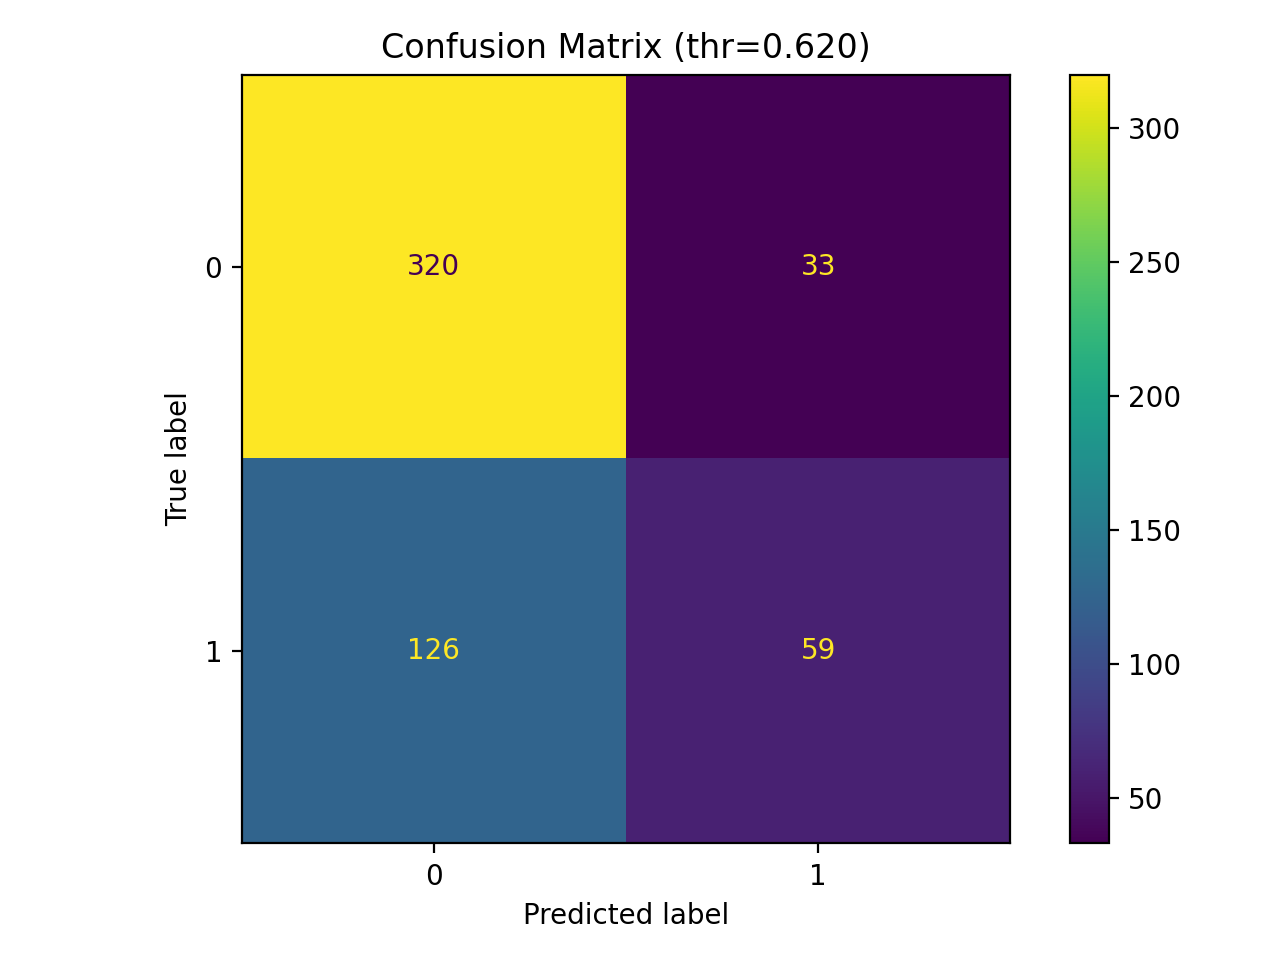
\includegraphics[width=0.75\linewidth]{figures/baseline/confusion_matrix_thr_spec0.90.png}
  \caption{Baseline confusion matrix at the specificity-constrained threshold (thr $\approx 0.620$).}
  \label{fig:cm_baseline}
\end{figure}

Figure~\ref{fig:roc_baseline} presents the receiver operating characteristic (ROC) curve for the baseline
model. The ROC--AUC of approximately 0.745 indicates that the classifier demonstrates reasonable
discriminative ability, performing substantially better than random chance. However, AUC alone does not
fully capture clinical usefulness in imbalanced datasets, motivating the inclusion of additional evaluation
metrics.

\begin{figure}[H]
  \centering
  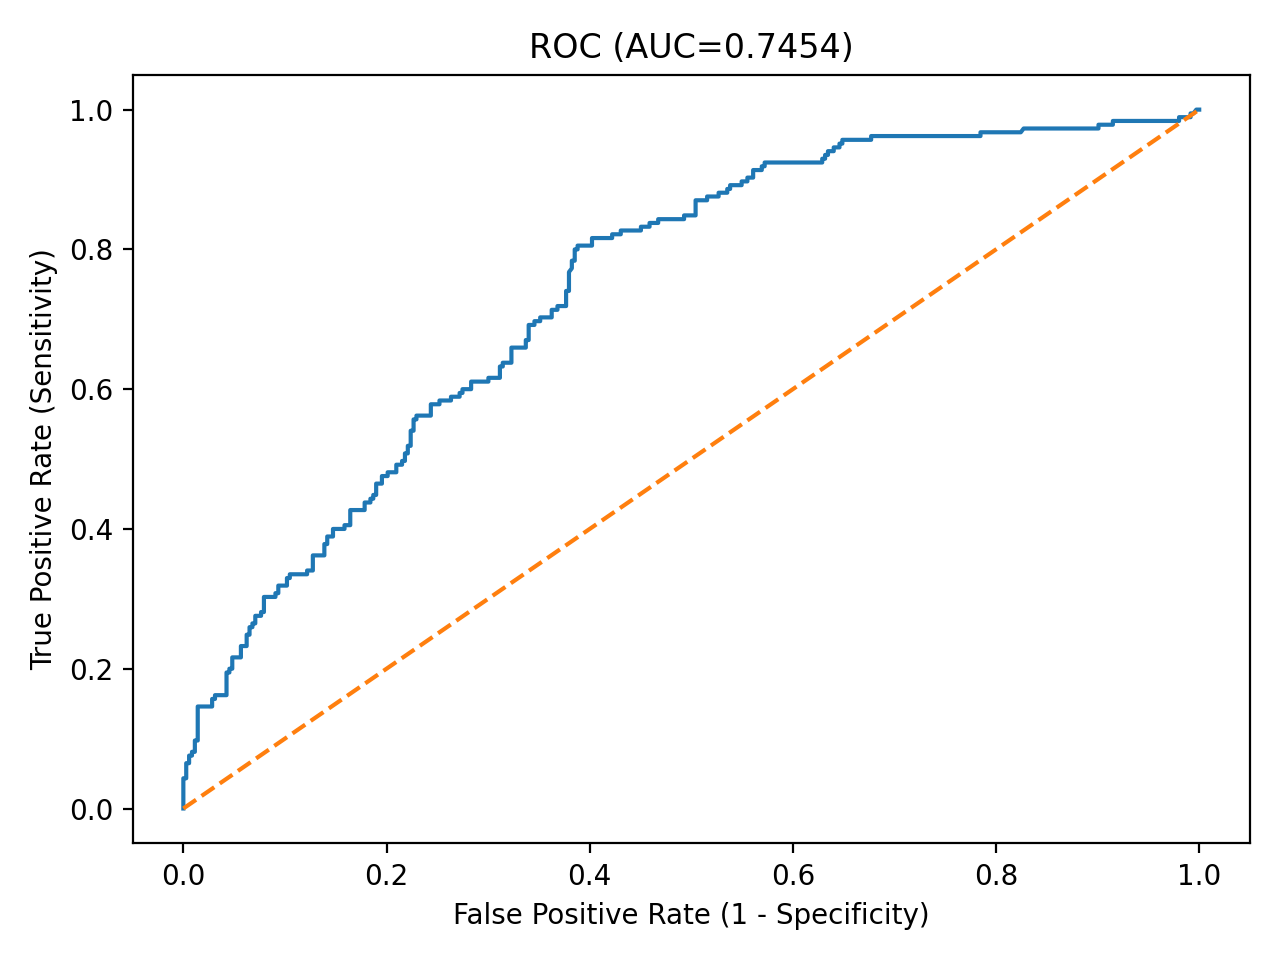
\includegraphics[width=0.75\linewidth]{figures/baseline/roc_curve.png}
  \caption{ROC curve for the baseline model (AUC $\approx 0.745$).}
  \label{fig:roc_baseline}
\end{figure}

The precision--recall (PR) curve is shown in Figure~\ref{fig:pr_baseline}. The average precision of
approximately 0.60 reflects the challenge of maintaining high precision while increasing recall in a
screening context where malignant cases are relatively rare. The PR curve provides a more informative
view of performance than ROC curves under class imbalance, particularly with respect to false positive
and false negative trade-offs.

\begin{figure}[H]
  \centering
  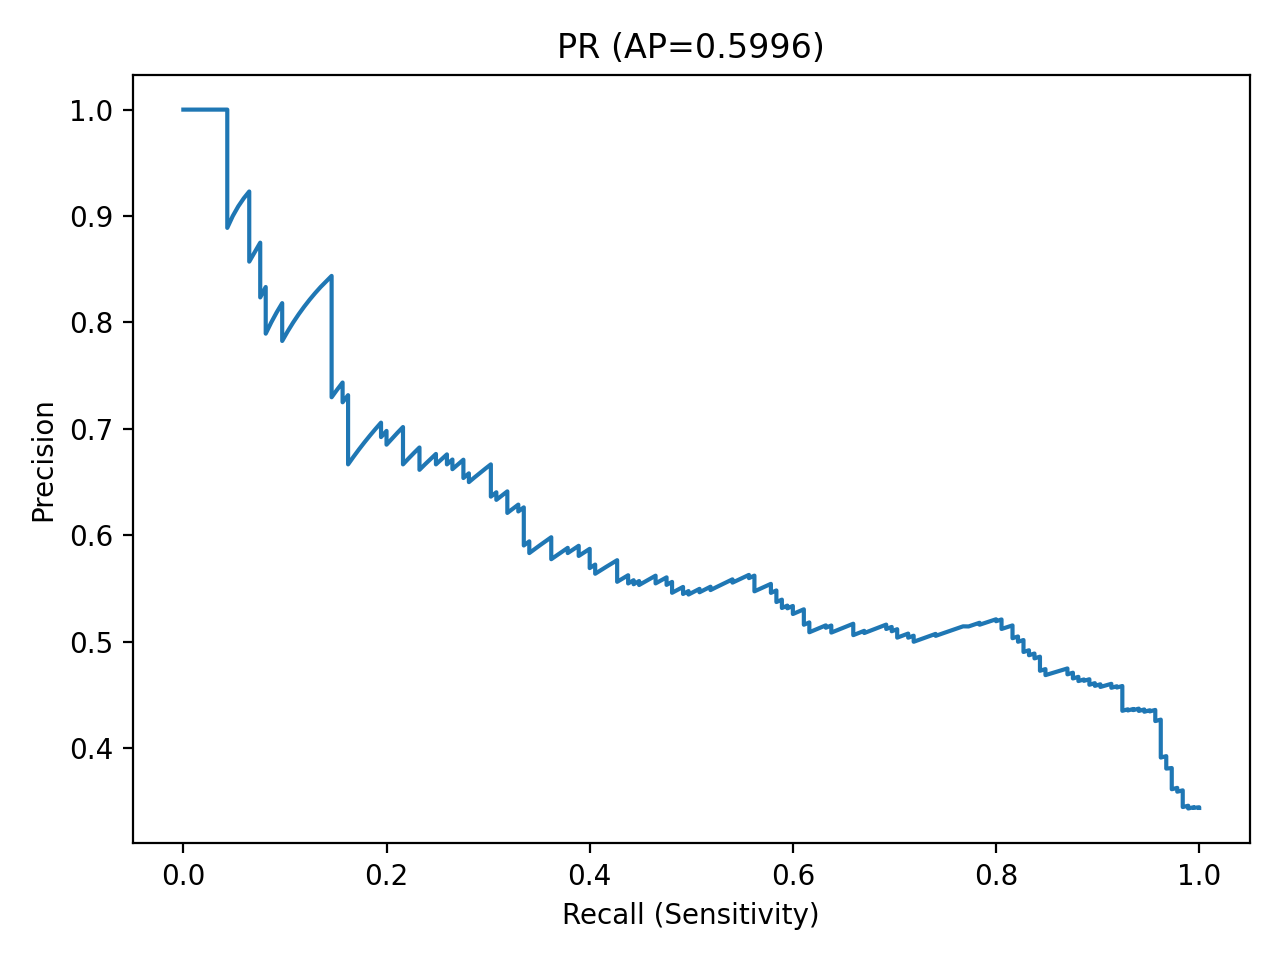
\includegraphics[width=0.75\linewidth]{figures/baseline/pr_curve.png}
  \caption{Precision--Recall curve for the baseline model (AP $\approx 0.600$).}
  \label{fig:pr_baseline}
\end{figure}

Finally, model calibration is assessed using the reliability diagram shown in
Figure~\ref{fig:cal_baseline}. While the predicted probabilities broadly follow the ideal diagonal trend,
deviations are visible across several bins, suggesting that the model is not perfectly calibrated. This
indicates that predicted confidence scores may not always correspond directly to true outcome
probabilities, which is an important consideration for human-in-the-loop deployment scenarios.

\begin{figure}[H]
  \centering
  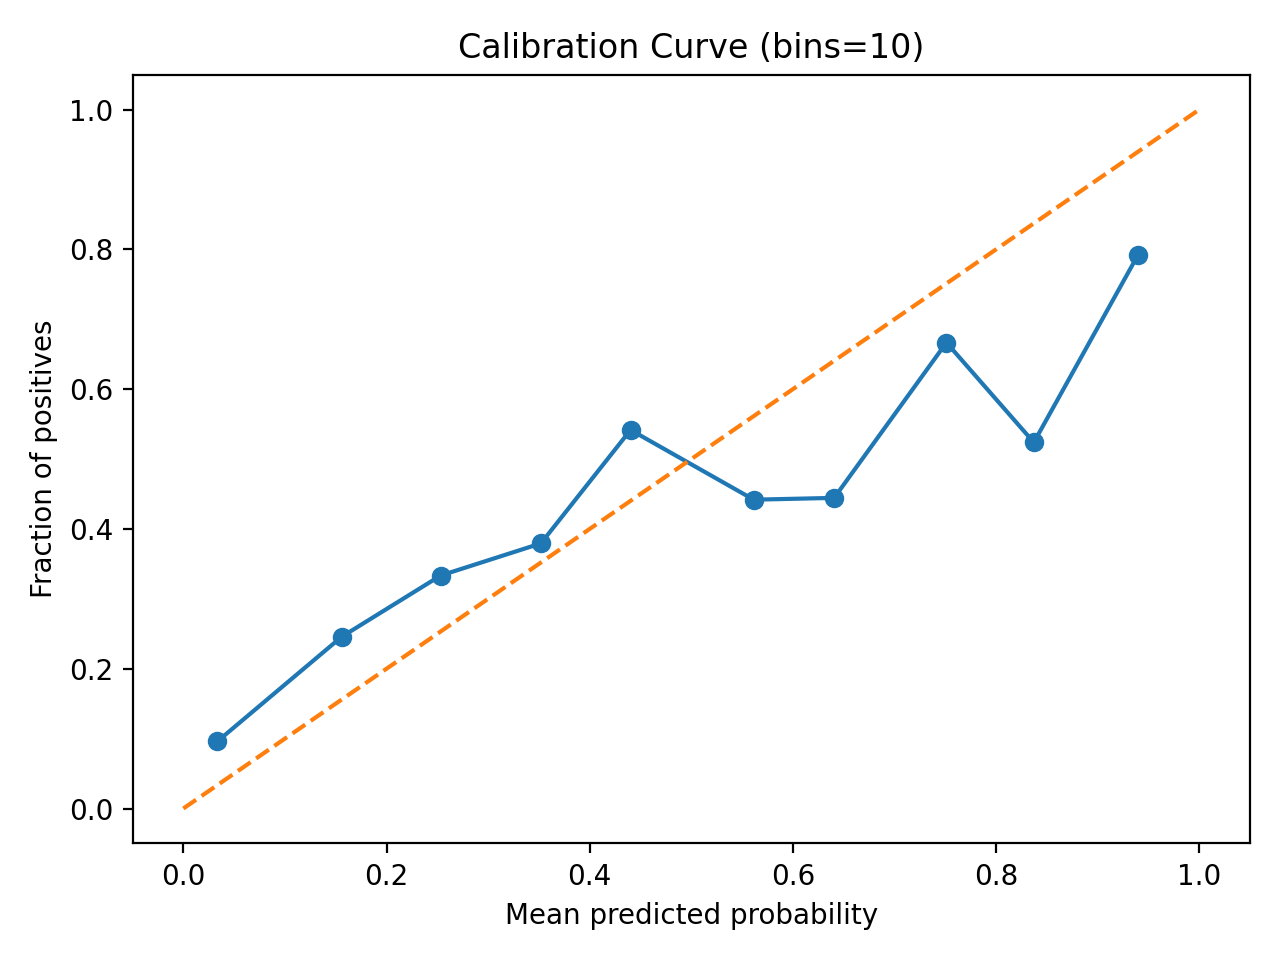
\includegraphics[width=0.75\linewidth]{figures/baseline/calibration_curve.png}
  \caption{Calibration curve for the baseline model (10 bins).}
  \label{fig:cal_baseline}
\end{figure}

Overall, these baseline results demonstrate that the proposed pipeline is capable of learning meaningful
discriminative features from mammography images, while also highlighting clear limitations in sensitivity
and calibration. These results establish a reference point against which subsequent architectural,
training, and evaluation refinements can be compared.
